\documentclass[times, utf8, zavrsni, numeric]{fer}
\usepackage{booktabs}
\usepackage{listings}
\usepackage{color}
\usepackage{xcolor}
\usepackage{enumitem, hyperref}
\usepackage{wrapfig}
\usepackage{float}
\usepackage{subcaption}
\captionsetup{singlelinecheck=on}
\captionsetup{justification=centering}
\usepackage{footnote}

\DeclareCaptionFont{white}{\color{white}}
\DeclareCaptionFormat{listing}{%
  \parbox{\textwidth}{\colorbox{gray}{\parbox{\textwidth}{#1#2#3}}\vskip-4pt}}
\captionsetup[lstlisting]{format=listing,labelfont=white,textfont=white}
\lstset{frame=lrb,xleftmargin=\fboxsep,xrightmargin=-\fboxsep,language=[LaTeX]{TeX},columns=flexible}
\renewcommand{\lstlistingname}{Kod}


\begin{document}

% TODO: Navedite broj rada.
\thesisnumber{3135}

% TODO: Navedite naslov rada.
\title{Inverzna perspektivna transformacija slike ravninskog objekta}

% TODO: Navedite vaše ime i prezime.
\author{Mak Krnic}

\maketitle

% Ispis stranice s napomenom o umetanju izvornika rada. Uklonite naredbu \izvornik ako želite izbaciti tu stranicu.
\izvornik

% Dodavanje zahvale ili prazne stranice. Ako ne želite dodati zahvalu, naredbu ostavite radi prazne stranice.
\zahvala{}

\tableofcontents

\chapter{Uvod}
\label{ch:uvod}
Uvod rada. Nakon uvoda dolaze poglavlja u kojima se obrađuje tema.

\chapter{Projekcijsko ravninsko preslikavanje}
\label{ch:preslikavanje}

\section{Prikaz točaka u ravnini homogenom notacijom}
\label{sec:homNot}

Svaka točka u ravnini u pravokutnom koordinatnom sustavu jednoznačno je određena uređenim parom koordinata $(x, y)$ te je stoga uobičajeno ravninu poistovjetiti s $\mathbb{R}^2$. Zbog toga se točku u ravnini može prikazati vektorom $\mathbf{x} = (x, y)^\top$.

Kao što se točka u ravnini može jednoznačno predstaviti  parom koordinata $(x,~y)$, tako se pravac može prikazati jednadžbom $ax + by + c = 0$, gdje se različiti pravci dobivaju mijenjajući parametre $a$, $b$ i $c$. Zbog tog se svojstva pravci mogu bez promjene mogu prikazati u homogenoj notaciji kao stupčani vektor $(a, b, c)^\top$. Ovaj prikaz, doduše, nije jednoznačan, budući da vektori $(a, b, c)$ i $(ka, kb, kc)$ predstavljaju isti pravac za svaki $k \neq 0$, ali za svaki pravac zapisan u homogenoj notaciji postoji točno jedan pravac zapisan u ortogonalnoj notaciji \citep{Hartley2004}.

Da bi se točka $\mathbf{x} = (x, y)^\top$ zapisala pomoću homogenih koordinata, potrebno je uzeti u obzir slijedeće:
\begin{enumerate}
	\item \label{itm:fst} Ako i samo ako točka $\mathbf{x} = (x, y)^\top$ leži na pravcu $\mathbf{I} =(a, b, c)^\top$, onda vrijedi jednakost $ax + by + c = 0$.
	\item Tvrdnja iz točke \ref{itm:fst} se može zapisati kao skalarni produkt vektora koji prikazuje točku i homogenog prikaza pravca: $(x, y, 1) \cdot (a, b, c) = (x, y, 1) \cdot \mathbf{I} = 0$.
	\item Ako i samo ako vrijedi $(x, y, 1) \cdot \mathbf{I} = 0$, onda vrijedi i  $(kx, ky, k) \cdot \mathbf{I} = 0$ za bilo koju konstantu $k \neq 0$.
\end{enumerate}

Iz gorenavedenoga vidi se da će točki $\mathbf{x} = (x_1, x_2, x_3)^\top$ iz projekcijske ravnine $\mathbb{P}^2$ odgovarati točka $(\frac{x_1}{x_3}, \frac{x_2}{x_3})^\top$ u euklidskoj ravnini $\mathbb{R}^2$, gdje je $x_3$ homogena koordinata točke $\mathbf{x}$.

Bitno je također napomenuti da se u slučaju kada je homogena koordinata točke $\mathbf{x}$ jednaka $0$ kaže da je ta točka u euklidskoj ravnini u beskonačnosti.

Projekcijski prostor $\mathbb{P}^2$ opisuje se kao skup zraka u prostoru $\mathbb{R}^3$. Ako se kroz ishodište prostora $\mathbb{R}^3$ provuče pravac, točke koje se nalaze na tom pravcu mogu se predstaviti vektorima $k(x_1, x_2, x_3)$ koji se u projekcijskom prostoru $\mathbb{P}^2$ preslikavaju u istu točku.

\section{Projekcijsko preslikavanje}
\label{sec:projPresl}

Planarna projekcijska transformacija ili \textit{homografija} je linearna transformacija nad homogenim 3-dimenzionalnim vektorom koji predstavlja homogeni zapis točke ravnine, a koja se može prikazati nesingularnom $3 \times 3$ matricom \citep{Hartley2004}:
\begin{equation}
	\label{eq:transLong}
	\left[\begin{matrix}
		x'_1 \\
		x'_2 \\
		x'_3
	\end{matrix}
	\right] \sim \left[\begin{matrix}
		h_{11} & h_{12} & h_{13} \\
		h_{21} & h_{22} & h_{23} \\
		h_{31} & h_{32} & h_{33}
	\end{matrix}
	\right]
	\cdot
	\left[
	\begin{matrix}
		x_1 \\
		x_2 \\
		x_3
	\end{matrix}
	\right]
\end{equation}
ili kraće
\begin{equation}
	\mathbf{x'} \sim H \cdot \mathbf{x}
	\label{eq:transShort}
\end{equation}

Važno je još primjetiti da se projekcijska transformacija ne mijenja skaliranjem transformacijske matrice $H$ faktorom različitim od nule, pa se zbog toga matrica $H$ naziva \textit{homogenom matricom} jer je bitan samo omjer elemenata, ali ne i same njihove vrijednosti. Budući da postoji 8 međusobno nezavisnih omjera, kažemo da projekcijska transformacija ima 8 stupnjeva slobode.

\section{Interpolacija}
\label{sec:interpolacija}

Interpolacija je matematička metoda kojom se na tememlju poznatog diskretnog skupa funkcijskih vrijednosti konstruiraju nove funkcijske vrijednosti. Diskretni se skup vrijednosti dobiva eksperimentalno ili uzorkovanjem te se interpolacija koristi kao jedna od metoda za rekonstruiranje funkcije. \citep{_interpolation_2013}

Osim linearne i bilinearne interpolacije za interpolaciju slikovnih elemenata postoje i druge metode interpolacije kao što su polinomna, \emph{spline}, interpolacija Gaussovim procesom, interpolacija racionalnim funkcijama i trigonometrijska. Navedene interpolacije pružaju određene prednosti nad linearnom i bilinearnom, ali presložene da bi se mogle izvršavati dovoljno brzo te je zato za ovaj rad odabrana bilinearna interpolacija.

\subsection{Linearna interpolacija}
\label{subsec:linInt}
\label{interpolation:lin}

Linearna interpolacija jedna je od najjednostavnijih metoda interpolacije namjenjen interpolaciji točaka sa samo jednom prostornom dimenzijom, odnosno za procjenu vrijednosti funkcije koja ovisi samo o jednom parametru. 

Pozunajući točke $A (x_1, y_1)$ i $B (x_2, y_2)$, linearni interpolant je dužina koja spaja te dvije točke. Pravac na kojem ta dužina leži izračunava se prema formuli za pravac kroz dvije točke \citep{_linear_2013}
\begin{equation}
	y = y_1 + (y_2 - y_1) \frac{x - x_1}{x_2 - x_1}, y_n = f(x_n)
\end{equation}

Linearna interpolacija nad skupom točaka dobiva se konkatenacijom pojedinih linearnih interpolacija između svakog para točaka, te je tada rezultat linearne interpolacije neprekinuta krivulja čija derivacija ima prekide u poznatim točkama \citep{Bosilj2010} \citep{_linear_2013}.

\subsection{Bilinearna interpolacija}
\label{subsec:bilinInt}

Bilinearna interpolacija je proširenje linearne interpolacije \ref{interpolation:lin}, a koristi se za interpolaciju funkcije dvije varijable na pravokutnoj 2D mreži. Provodi se tako da se provede \textbf{linearna} interpolacija prvo u jednom smjeru, a zatim u drugom \citep {_bilinear_2013}. Nije bitno koji je smjer prvi.

Ako su nam poznate vrijednosti funkcije u točkama $Q_{11} (x_1, y_1)$, $Q_{12} (x_1, y_2)$, $Q_{21}  (x_2, y_1)$ i $Q_{22} (x_2, y_2)$, onda bilinearnom interpolacijom možemo naći nepoznatu vrijednost funkcije $f$ u točki $P (x, y)$ koja se nalazi unutar pravokutnika omeđenog točkama $Q_{11}$, $Q_{12}$, $Q_{21}$ i $Q_{22}$.

Na slici \ref{fig:bilintPrikaz} se može vidjeti grafički prikaz izračuna vrijednosti interpolirane točke.

\begin{figure}[ht]
\centering
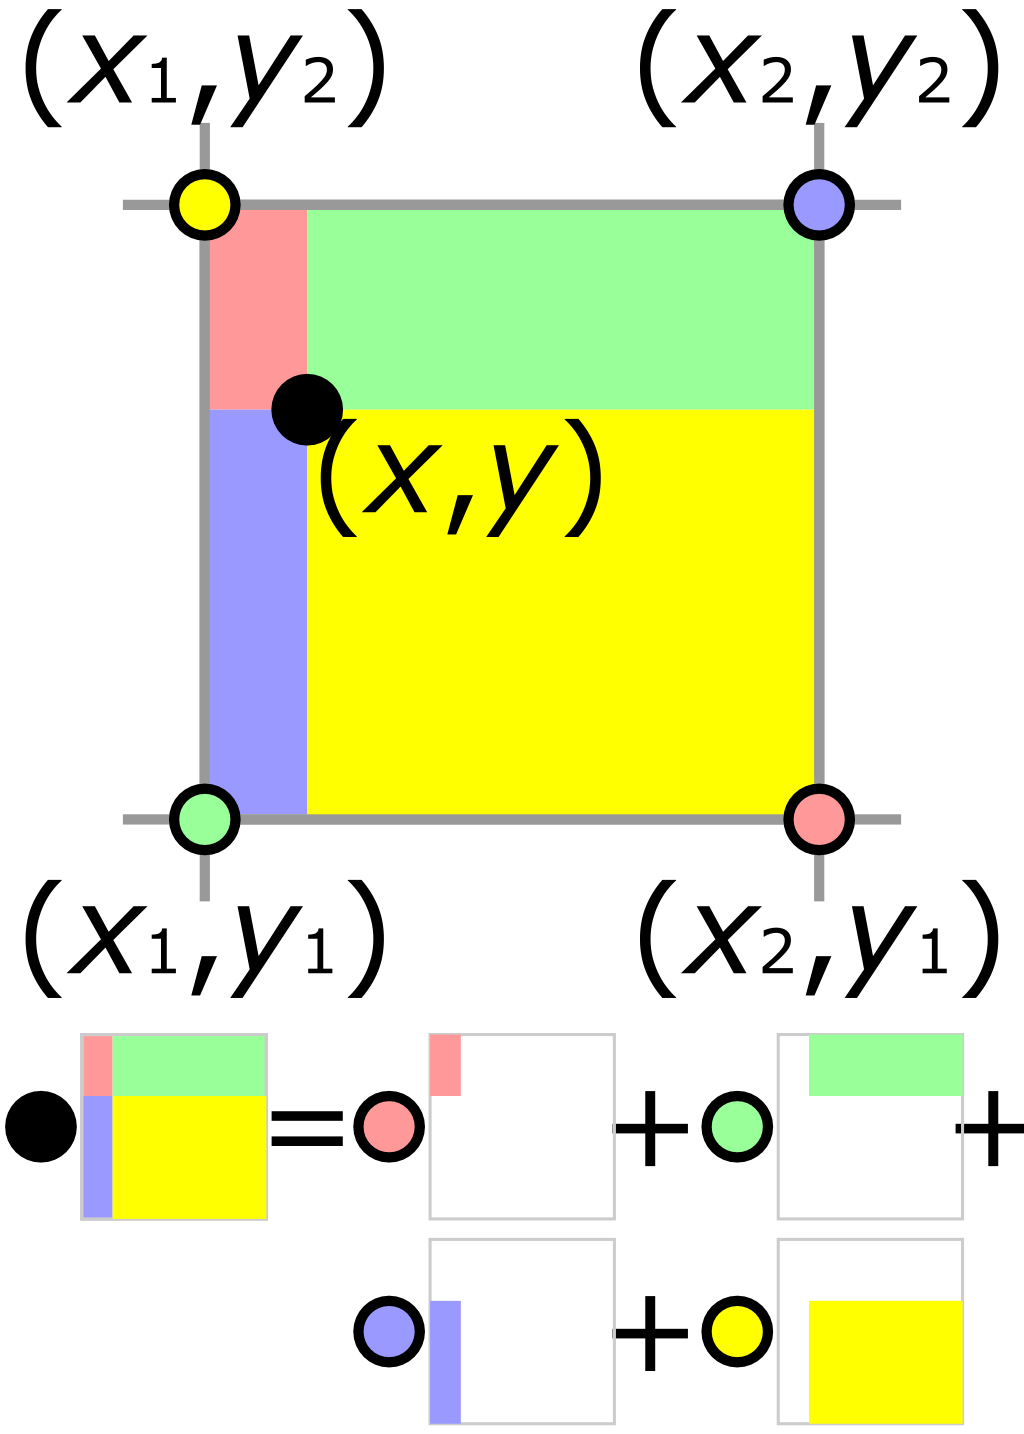
\includegraphics[width=6cm]{figures/bilint_visualization.png}
\caption{Grafički prikaz bilinearne interpolacije}
\label{fig:bilintPrikaz}
\end{figure}

Za primjer, pokazat ćemo algoritam kada se linearna interpolacija radi prvo po $x$-osi, a zatim po $y$-osi.
\begin{equation}
f(R_1) \approx \frac{x_2 - x}{x_2 - x_1} f(Q_{11}) + \frac{x - x_1}{x_2 - x_1} f(Q_{21})\text{ ,}
\end{equation}
gdje je  $R_1 = (x, y_1)$.
\begin{equation}
f(R_2) \approx \frac{x_2 - x}{x_2 - x_1} f(Q_{12}) + \frac{x - x_1}{x_2 - x_1} f(Q_{22})\text{ ,}
\end{equation}
gdje je  $R_2 = (x, y_2)$.

Zatim nastavljamo provodeći interpolaciju po $y$-smjeru:
\begin{equation}
f(P) \approx \frac{y_2 - y}{y_2 - y_1} f(R_1) + \frac{y - y_1}{y_2 - y_1} f(R_2).
\end{equation}

Potrebno je skrenuti pozornost na to da se u degeneriranom slučaju bilinearne transfomacije kada se provodi nad jednodimenzionalnom slikom spada na linearnu interpolaciju koja se provodi samo u smjeru u kojem se proteže ta jedna dimenzija.

Iako se ova metoda interpolacije naziva \emph{bilinearna} i svaki korak jest linearan, to je ustvari umnožak dvije linearne funkcije, odnosno to je kvadratna funkcija oblika:
\begin{equation}
	(a_1x + a_2)(a_3y + a_4) \text{.}
\end{equation}

U ovom se radu bilinearna interpolacija koristi za određivanje boje slikovnog elementa \engl{pixel} u slučaju kada originalne koordinate transformirane točke nisu cjelobrojne, te se zbog toga može koristiti pojednostavljena verzija algoritma u kojoj se pretpostave koordinate točaka $(0,0)$, $(0, 1)$, $(1, 0)$ te $(1, 1)$:
\begin{equation}
\label{eq:interpolationSImple}
f(x, y) \approx f(0, 0)(1 - x)(1 -  y) + f(1, 0) x (1 - y) + f(0, 1) (1 - x) y + f(1, 1) x y
\end{equation}

\section{Singularna dekompozicija}
\label{sec:svd}

Singularna dekompozicija matrice je tehnika koja veoma bitna za rješavanje problema u području računalnog vida. Među ostalime, koristi se, kao u ovom radu, za izračunavanje skupa homogenih linearnih jednadžbi $A\mathbf{x}=\mathbf{0}$.

Svaka se realna matrica $A_{m \times n}$ može zapisati kao produkt triju matrica:
\begin{equation}
	A = U D V^\top
\end{equation}
gdje su $U_{m \times m}$ i $V_{n \times n}$ matrice čiji su stupci međusobno okomiti jedinični vektori, a $D_{m \times n}$ je dijagonalna matrica čiji se elementi dijagonale $\sigma_i$ nazivaju singularne vrijednosti i vrijedi $\sigma_1 \geq \sigma_2 \geq \ldots \sigma_n \geq 0$.

\section{Određivanje transformacijske matrice}
\label{sec:odredjivanjeTransMat}

Ako su nam poznate koordinate četiriju točaka na originalnoj slici $I_o$ te znamo u koje se one točke preslikavaju na transformiranoj slici $I_t$, može se riješiti jednadžba \eqref{eq:transShort} i na taj način dobiti transformacijsku matricu $H$ \citep{segvicDinAn3D}.

S obzirom na to da nam činjenica da se transformacijska matrica $H$ može množiti koeficijentom uvelike komplicira situaciju, kako bi pojednostavili jednadžbu \eqref{eq:transShort} za svaku točku, možemo je zapisati na slijedeći način:
\begin{equation}
q_t = \lambda \cdot H \cdot q_o, \lambda \in \mathbb{R}
\label{eq:transMatSimpler}
\end{equation}
gdje je $q_t$ transformirana točka, a $q_o$ originalna.

Nadalje, iz jednadžbe \eqref{eq:transMatSimpler} se može iščitati da su $q_t$ i $H \cdot q_o$ paralelni, što znači da je njihov vektorski produkt jednak $\mathbf{0}$ \citep{vecParallel}:
\begin{equation}
\label{eq:crossProd}
q_t \times (H \cdot q_o) = \vec{0}
\end{equation}
Radi jednostavnijeg zapisa jednadžbi \eqref{eq:transLong} i \eqref{eq:transShort} možemo reći da retke matrice $H$ prikazujemo retčanim vektorima $h_i$.:
\begin{equation}
H = \left[
\begin{matrix}
h_{11} & h_{12} & h_{13} \\
h_{21} & h_{22} & h_{23} \\
h_{31} & h_{32} & h_{33}
\end{matrix}
\right]
= \left[
\begin{matrix}
\mathbf {h_1} \\
\mathbf{h_2} \\
\mathbf{h_3}
\end{matrix}
\right]
\end{equation}
Tada dalje \eqref{eq:crossProd} postaje
\begin{equation}
\label{eq:transCrossProdLong}
\mathbf{q_t} \times \left[
\begin{matrix}
\mathbf {h_1} \cdot \mathbf{q_o} \\
\mathbf{h_2} \cdot \mathbf{q_o} \\
\mathbf{h_3} \cdot \mathbf{q_o}
\end{matrix}
\right]
= \left[
\begin{matrix}
q_{tx} \\
q_{ty} \\
q_{tz}
\end{matrix}
\right]
\times \left[
\begin{matrix}
\mathbf {h_1} \cdot \mathbf{q_o} \\
\mathbf{h_2} \cdot \mathbf{q_o} \\
\mathbf{h_3} \cdot \mathbf{q_o}
\end{matrix}
\right]
= \mathbf{0}
\end{equation}

Budući da su i transformirana ($q_t$) i originalna ($q_o$) točka zadane u ortogonalnoj notaciji, njihove su homogene koordinate $q_{tz}$ i $q_{oz}$ jednake $1$ te \eqref{eq:transCrossProdLong} postaje:
\begin{equation}
\label{eq:transCrossProdDetailed}
\left[
\begin{matrix}
q_{tx} \\
q_{ty} \\
1
\end{matrix}
\right]
\times \left[
\begin{matrix}
\mathbf{h_1} \cdot \mathbf{q_o} \\
\mathbf{h_2} \cdot \mathbf{q_o} \\
\mathbf{h_3} \cdot \mathbf{q_o}
\end{matrix}
\right]
= \left[
\begin{matrix}
q_{ty} \cdot \mathbf{h_3} \cdot \mathbf{q_o} - \mathbf{h_2} \cdot \mathbf{q_o} \\
-q_{tx} \cdot \mathbf{h_3} \cdot \mathbf{q_o} + \mathbf{h_1} \cdot \mathbf{q_o} \\
q_{tx} \cdot \mathbf{h_2} \cdot \mathbf{q_o} + q_{ty} \cdot \mathbf{h_1} \cdot \mathbf{q_o}
\end{matrix}
\right]
= \mathbf{0}
\end{equation}
Nakon što izlučimo $\mathbf{h_1}$, $\mathbf{h_2}$ i $\mathbf{h_3}$ dobivamo:
\begin{equation}
\left[
\begin{matrix}
0 & 0 & 0 & -q_{ox} & -q_{oy} & -1 & q_{ty} q_{ox} & q_{ty} q_{oy} & q_{ty} \\
q_{ox} & q_{oy} & 1 & 0 & 0 & 0 & -q_{tx} q_{ox} & -q_{tx} q_{oy} & -q_{tx} \\
-q_{ty} q_{ox} & -q_{ty} q_{oy} & -q_{ty} & q_{tx} q_{ox} & q_{tx} q_{oy} & q_{tx} & 0 & 0 & 0
\end{matrix}
\right]
\cdot
\left[
\begin{matrix}
h_{11} \\
h_{12} \\
h_{13} \\
h_{21} \\
h_{22} \\
h_{23} \\
h_{31} \\
h_{32} \\
h_{33}
\end{matrix}
\right]
\end{equation}
ili kraće
\begin{equation}
\left[
\begin{matrix}
\mathbf{0}_3^\top & -\mathbf{q_o}^\top & q_{ty} \mathbf{q_o}^\top \\
\mathbf{q_o}^\top & \mathbf{0}_3^\top & -q_{tx} \mathbf{q_o}^\top \\
-q_{ty}\mathbf{q_o}^\top & q_{tx} \mathbf{q_o}^\top & \mathbf{0}_3^\top
\end{matrix}
\right]
\cdot
\left[
\begin{matrix}
\mathbf{h_1}^\top \\
\mathbf{h_2}^\top \\
\mathbf{h_3}^\top
\end{matrix}
\right]
= \mathbf{0}_3
\end{equation}

Za svaki par točaka dobivamo po dvije nezavisne jednadžbe, dakle, za četiri para dobivamo linearni sustav oblika:
\begin{equation}
\label{eq:transSystemShort}
A_{8\times9} \cdot \mathbf{h}_{9\times1} = \mathbf{0}_{8\times1}
\end{equation}
Uočavamo da sustav iz \eqref{eq:transSystemShort} ima 8 jednadžbi i 9 nepoznanica. Taj je sustav moguće rješiti zahvaljujući njegovom svojstvu homogenosti\footnote{Homogen sutstav je sustav oblika $A\mathbf{x} = \mathbf{0}$} metodom singularne dekompozicije \engl{SVD, singular value decomposition}.

\chapter{Programska implementacija}
\label{ch:implementacija}

\section{Prototip u pythonu}
\label{sec:pythonProto}

\section{Implementacija u C++-u}
\label{sec:implC++}
\lstset{language=C++, tabsize=2}
\begin{lstlisting}
int main () {
	return 0;
}
\end{lstlisting}
\chapter{Korištena programska podrška i biblioteke}
\section{Python}
\subsection{Python Imaging Library (PIL)}
\subsection{pylab}
\subsection{numpy}

\section{C++}
\subsection{OpenCV}
\chapter{Rezultati}
\label{ch:rezultati}
\chapter{Zaključak}
\label{ch:zakljucak}

U okviru ovog rada ostvaren je postupak izračuna transformacijske matrice perspektivne transformacije na temelju korisničkog odabira četiriju točaka. Drugi dio rada se bavi perspektivnom transformacijom pomoću matrice dobivene u prvom koraku. Pokazalo se da za obradu slike u stvarnom vremenu (a što je potrebno u slučaju npr. ispravljanja perspektive slike snimane kamerom montiranom na vozilo za vrijeme vožnje) nije dostatan jezik Python već se zadovoljavajući rezultati postižu korištenjem C++-a. Također rezultati su pokazali da se ubrzanje od oko 25-35\% može postići isključivanjem interpolacije. 

Daljnji rad i istraživanje bi se moglo kretati u smjeru olakšavanja korisničkog unosa referentnih točaka, kako je već navedeno u rezultatima. Također, mogle bi se iskoristiti alternativne metode interpolacije za bolje rezultate. Dodatna ubrzanja mogla bi se postići daljnjim optimiziranjem algoritma preslikavanja točaka iz originalne u transformiranu sliku.

\bibliographystyle{fer}
\bibliography{literatura}

\begin{sazetak}

U ovom radu implementiran je algoritam za izračun matrice inverzne perspektivne transformacije na temelju korisničkog unosa četiri točke. Inverzna perspektivna transformacija je važan postupak područja računalnog vida s raznim primjenama. Za potrebe izračuna matrice proučena je matematička metoda singularne dekompozicije \engl{SVD}, a za samu implementaciju biblioteka \emph{OpenCV} za C++ te biblioteke \emph{Python Imaging Library}, \emph{PyLab} i \emph{NumPy} za Python. Provedena su testiranja i usporedbe vremena izvođenja te je utvrđeno da se implementacija u C++-u izvodi višestruko brže od implementacije u Pythonu te da je implementacija u C++-u pogodna za obradu slike u stvarnom vremenu.

\kljucnerijeci{projekcijsko ravninsko preslikavanje, homografija, projekcijska transformacija, računalni vid, obrada slike, izračun matrice homografije}
\end{sazetak}

% TODO: Navedite naslov na engleskom jeziku.
\engtitle{Inverse perspective mapping of a planar object}
\begin{abstract}

This work implements the algorithm for the calculation of the inverse perspective transformation matrix based on user-selected four points. Inverse perspective mapping is an important method in the field of computer vision with various applications. For the matrix computation attention was given to the method of singular value decomposition, and for the implementation itself \emph{OpenCV} library for C++ and the libraries \emph{Python Imaging Library (PIL)}, \emph{PyLab} and \emph{NumPy} for Python. The testing was conducted noting execution times and it has been noticed that the C++ implemtation's execution time is many times shorter than that of Python's and that the C++ implementation is suitable for real-time image processing.

\keywords{projective planar mapping, homography, projective transformation, computer vision, image processing, homography matrix calculation}
\end{abstract}

\end{document}
